\chapter{Studi Literatur}

Pada bab ini, Penulis akan menguraikan hasil studi literatur dalam penyusunan
tugas akhir ini. Subbab pertama membahas trem, yaitu kendaraan yang akan
disimulasikan menjadi otonom pada tugas akhir ini. Selanjutnya, akan dibahas
simulator CARLA, yaitu perangkat lunak yang digunakan sebagai alat simulasi.
Subbab ketiga menjelaskan NVIDIA Pegasus yang akan digunakan sebagai mesin untuk
menjalankan algoritma \textit{decision making} di lingkungan simulasi dan
\textit{production}. Lalu, subbab keempat akan membahas NVIDIA DriveWorks
sebagai SDK (\textit{software development kit}) pengembangan perangkat lunak
pada NVIDIA Pegasus. Lalu, pada subbab kelima akan dibahas kondisi metode
komunikasi jalur komunikasi serta ZeroMQ dan ROS2 sebagai alternatif ke kondisi
yang ada. Terakhir, subbab keenam akan membahas penelitian-penelitian terkait
simulasi \textit{autonomous vehicle} menggunakan CARLA.

\section{Trem}

Trem adalah transportasi umum berupa kereta ringan yang memiliki rel/jalur
sendiri di jalan raya. Trem dapat menjadi solusi terhadap masalah yang semakin
besar di kota-kota besar, yaitu kemacetan dan polusi. Hal ini karena trem dapat
memuat lebih banyak penumpang daripada mobil biasa. Lalu, kebanyakan trem
menggunakan listrik sehingga tidak ada emisi karbon dioksida di kota dan tidak
banyak mengeluarkan suara.

Di Indonesia sendiri, trem sudah ada sejak jaman penjajahan. Trem banyak
digunakan di Ibu Kota Negara, Jakarta, sampai 15 April 1954. Untungnya, trem
masih banyak digunakan di daerah Madiun dan Solo.

Tugas akhir ini adalah bagian dari proyek pengembangan trem otonom. Trem otonom
yang dikembangkan menggunakan basis trem di Kota Solo dan Kota Madiun. Trem
otonom, secara teori, tidak membutuhkan masinis untuk mengoperasikannya.
Pengereman dan percepatan trem dikendalikan program kecerdasan buatan. Tugas
akhir ini akan menggunakan trem otonom virtual yang dijalankan pada dunia
simulasi. Dengan simulasi, algoritma kendali dapat diuji tanpa adanya risiko
kecelakaan serta tanpa harus menyewa trem.

\section{Simulator CARLA}

CARLA (\textit{Car Learning to Act}) adalah perangkat lunak sumber terbuka
(\textit{o\-pen sour\-ce}) yang memiliki tujuan utama menyimulasikan kendaraan
autonomous. CAR\-LA dibangun dari nol untuk mampu melakukan pelatihan, pembuatan
prototipe, dan validasi model kemudi otonom, termasuk persepsi dan kontrol dari
model tersebut \parencite{dos_carla}.

\begin{figure}[h!]
    \centering
    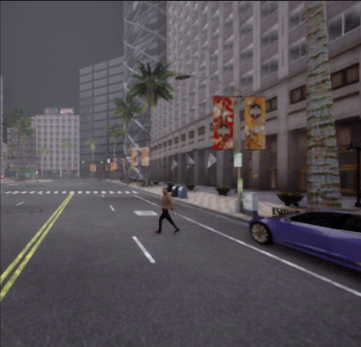
\includegraphics[width=0.5\textwidth]{resources/chapter-2/CARLA-cropped.png}
    \caption{Antarmuka simulator CARLA}
\end{figure}

CARLA sendiri dibangun di atas mesin gim (\textit{game engine}) Unreal Engine 4
(UE4). UE4 dipilih karena memiliki simulasi fisika dan kualitas grafis terbaik,
setidaknya pada saat CARLA dibuat. Selain itu, UE4 juga memiliki ekosistem untuk
pengaya (\textit{plugin}) dan sistem untuk menambahkan logika dasar untuk
(\textit{non-playable character}\footnote{Istilah untuk karakter yang tidak
    dapat dimainkan pada gim.}). UE4 dan sifat sumber terbuka CARLA memungkinkan
komunitas untuk menambahkan berbagai hal sesuai dengan kebutuhan mereka atau
bahkan memperbaiki CARLA.

Agar simulasi yang dilakukan CARLA serealistis mungkin, CARLA menyediakan
berbagai macam model 3D: kendaraan, pejalan kaki, gedung, dan rambu lalu lintas.
Model-model 3D yang disediakan dibuat dengan menggunakan teknik yang
menghasilkan bentuk dan tekstur senyata mungkin, akan tetapi tetap cepat untuk
di-\textit{render}. Model kendaraan dan pejalan kaki yang dibuat bisa memiliki
banyak variasi, misalnya kendaraan Yamaha YZF dengan warna yang berbeda atau
pejalan kaki dengan aksesoris dan pakaian yang berbeda. Model-model 3D
digunakan untuk membangun lingkungan simulasi yang realistis.

Selain dari model 3D, lingkungan simulasi yang realistis didapatkan juga dari
cuaca dan waktu hari. Cuaca dan waktu hari pada CARLA dapat dikustomisasi
se\-de\-mi\-ki\-an rupa untuk memungkinkan berbagai macam skenario simulasi.
Selain itu, NPC yang ada di CARLA akan menggunakan sebuah model dari kendaraan
ataupun pejalan kaki. NPC bergerak berdasarkan suatu aturan yang sudah
ditentukan, misalnya mengikuti suatu pemilihan keputusan ketika di lampu lalu
lintas.

Selain model, CARLA juga menyediakan berbagai sensor untuk menyimulasikan
pengambilan data. Sensor-sensor tersebut dapat ``ditempelkan'' ke kendaraan
simulasi. Contoh sensor yang tersedia adalah kamera dan LIDAR (\textit{Light
    Detection and Ranging}), dan lain-lain. Selain data dari sensor, bisa didapatkan
juga data seperti kecepatan dan percepatan (mirip dengan data dari GPS) dari
kendaraan.

CARLA bekerja dengan arsitektur server-klien. Arsitektur ini memungkinkan dunia
yang dinamis dan antarmuka yang sederhana antara dunia dan agen yang
berinteraksi dengannya. Server pada CARLA berfungsi untuk menjalankan simulasi
dan me-\textit{render scene}-nya. Lalu, klien bertugas untuk mengirimkan
perintah dan ``perintah meta'' ke server dan menerima data sensor. Perintah yang
dapat dikirimkan klien digunakan untuk mengendalikan kendaraan yang
disimulasikan. Sedangkan ``perintah meta'' digunakan untuk mengatur lingkungan
simulasi, misalnya cuaca, sensor yang digunakan, dan jumlah kendaraan/pejalan
kaki NPC.

Pada sistem simulasi tugas akhir, komponen klien dan server CARLA akan
dijalankan pada server SILS. Data yang didapatkan dari CARLA akan dikirim ke
server AGX/RKB untuk dikonsumi oleh program GRS (kendali). Klien CARLA akan
berkomunikasi dengan sebuah \textit{agent} dengan sebuah API Python sehingga
\textit{agent} dapat mendapatkan data dari CARLA dan mengirimkannya ke komputer
RKB/AGX.

\section{NVIDIA Pegasus}

NVIDIA Pegasus adalah salah satu produk cetusan NVIDIA Corporation di bawah lini
produk NVIDIA Drive PX. Nama pasar dari NVIDIA Pegasus adalah N\-VI\-DI\-A Drive
PX Pegasus. Lini produk NVIDIA Drive sendiri merupakan platform komputer untuk
memberikan fungsionalitas bantuan mengemudi pada kendaraan bermotor.

\begin{figure}[h!]
    \centering
    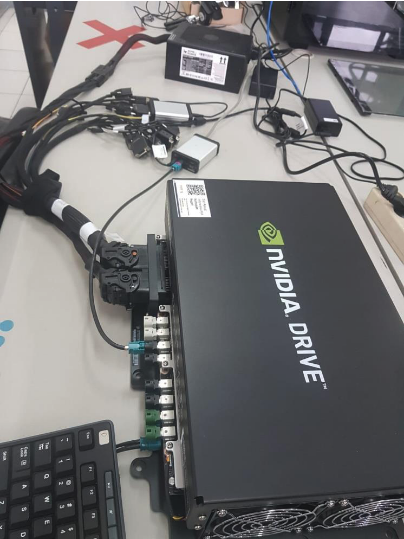
\includegraphics[width=\textwidth]{resources/chapter-2/pegasus.png}
    \caption{NVIDIA Pegasus \parencite{trilaksono_laporanRispro}}
\end{figure}

Mengutip dari \parencite{oh_2017}, NVIDIA Pegasus adalah komputer yang mendukung
pengemudian \textit{autonomous} secara penuh. Artinya, NVIDIA Pegasus dapat
digunakan untuk membuat sebuah kendaraan bermotor menjadi \textit{autonomous
    vehicle} jika sensor dan algoritma yang digunakan tepat.

NVIDIA Pegasus menggunakan 2 GPU dengan arsitektur post-Volta dan 2 SoC NVIDIA
Xavier. Kombinasi CPU dan GPU ini dapat menghasilkan 320 TOPS (\textit{trillion
    operations/second}) untuk komputasi intelegensi buatan. Untuk koneksi I/O,
NVIDIA Pegasus mendukung sampai dengan 16 kamera (6 di antaranya adalah lidar).

Karena NVIDIA Pegasus dapat dihubungkan langsung ke sensor, di produk akhir
sensor akan langsung dihubungkan pada NVIDIA Pegasus. Metode komunikasi yang
dibuat tidak akan digunakan pada produk akhir dan hanya digunakan untuk
kepentingan simulasi, terutama simulasi \textit{hardware-in-the-loop}.

Pada trem otonom, NVIDIA Pegasus akan digunakan untuk menjalankan program GRS
(kendali). Sehingga komputer ini juga akan digunakan untuk pengujian sebelum
digunakan pada produk akhir.

\section{NVIDIA DriveWorks}

NVIDIA DriveWorks adalah SDK (\textit{software development kit}) untuk
mengembang\-kan perangkat lunak yang digunakan pada kendaraan otonom dengan
perangkat keras dari NVIDIA AGX. NVIDIA DriveWorks menyediakan berbagai kakas yang
dapat  digunakan untuk mempercepat pengembangan algoritma dan perangkat lunak
untuk kendaraan otonom. Kemampuan dari NVIDIA DriveWorks juga dapat dikembangkan
lagi oleh pemrogram karena sifatnya yang modular, terbuka, dan
\textit{customizable} \parencite{nvidia_driveworksMainSite}.

NVIDIA DriveWorks sendiri sudah mencapai versi 5. Akan tetapi, pada tugas
akhir ini akan digunakan NVIDIA DriveWorks 4. NVIDIA DriveWorks 4 dapat
dijalankan pada perangkat keras  NVIDIA Pegasus dan juga pada GPU
\textit{desktop} NVIDIA dengan \textit{chip} Turing atau Volta, misalnya NVIDIA
RTX 20-\textit{series} \parencite{nvidia_driveworksSdkGettingStarted}.

Beberapa pustaka dan kakas yang disediakan NVIDIA DriveWorks adalah visualisasi
(GUI), pengoptimal TensorRT, lapisan abstraksi kendaraan, perkiraan
``egomotion'', perekam data, dan \textit{logging} dan diagnosis sistem. Selain
itu, beberapa fitur utama dari NVIDIA DriveWorks adalah
\begin{enumerate}
    \item lapisan abstraksi sensor: memberikan antarmuka yang sama untuk
        memanipulasi semua sensor yang didukung, kemampuan untuk membuat sensor
        virtual menggunakan data yang direkam, dan lain-lain;
    \item pemroses gambar dan \textit{point cloud} (data lidar): terdapat
        berbagai pemroses gambar seperti \textit{detection} dan
        \textit{tracking} dan pemroses \textit{point cloud} seperti segmentasi
        planar dengan abstraksi perangkat keras sehingga beberapa fitur
        pemrosesan dapat dipercepat pada NVIDIA Drive tertentu; dan
    \item kerangka kerja DNN (\textit{deep neural network}): kerangka kerja yang
        dapat digunakan untuk mamuat dan memprediksi menggunakan model ML
        TensorRT yang sudah di-\textit{train}.
\end{enumerate}

Pada tugas akhr ini, NVIDIA DriveWorks digunakan untuk membaca dan
memroses data-data sensor. Selain itu, sensor virtual pada NVIDIA DriveWorks
juga akan dimanfaatkan sebagai media untuk menyimpan data sensor yang dikirim
dari komputer SILS. Data dari komputer SILS akan dimuat secara langsung ke
memori perangkat sehingga oleh NVIDIA DriveWorks dianggap data dari
\textit{file} rekaman.

\section{Metode Komunikasi antara Simulator CARLA dan NVI\-DI\-A Pegasus}

Pada keadaan yang ada, komunikasi antara komputer SILS dengan komputer RKB/AGX
menggunakan perantara \textit{web service} yang berbasis HTTP (dapat dilihat
pada Gambar \ref{chapter-2-old-hils}). Penggunaan HTTP pada \textit{web service}
sendiri sebenarnya bukan \textit{bottleneck}/penghambat kinerja terbesar sistem
simulasi. \textit{Bottleneck} terbesar adalah operasi I/O yang dilakukan setiap
kali dilakukan pengiriman data. Dilakukan delapan operasi I/O yang berjalan
secara sinkronis untuk mengirimkan data. Operasi-operasi tersebut berbentuk
baca/tulis ke \textit{file} dan basis data serta permintaan HTTP.

\begin{figure}[h!]
    \centering
    \includegraphics[width=1.0\textwidth]{resources/chapter-2/komunikasi
        data pada simulasi.png}
    \caption{Arsitektur komunikasi pada HILS \parencite{trilaksono_laporanRispro}}
    \label{chapter-2-old-hils}
\end{figure}

Dampaknya dapat dilihat ketika dibandingkan dengan SILS (\textit{software
    in the loop simulation}, tanpa NVIDIA Pegasus) didapatkan kinerja 4000 transaksi
per detik. Sedangkan ketika menjadi HILS, hanya didapatkan 100--110 transaksi per
detik \parencite{trilaksono_laporanRispro}. Oleh karena itu, pada subbab ini
akan dibahas beberapa metode komunikasi alternatif yang dapat digunakan untuk
menyederhanakan arsitektur dan lebih cocok dengan kasus penggunaan sistem
simulasi. Alternatif-alternatif tersebut adalah ZeroMQ dan ROS. Kedua alternatif
dipilih karena CARLA mengirimkan sensor secara asinkron dan keduanya dinilai
lebih baik dalam menangani komunikasi asinkron daripada HTTP.

\subsection{ZeroMQ}

ZeroMQ adalah sebuah pustaka yang memberikan pe\-ning\-ka\-tan di atas
\textit{socket} tradisional. ZeroMQ memberikan fungsionalitas tambahan terhadap
\textit{socket} dan mengabstraksi pembuatan koneksi TCP dengan harapan
memudahkan pengembangan aplikasi terdistribusi. Fungsionalitas yang ditambahkan
oleh ZeroMQ didasarkan pada pola-pola komunikasi yang sering terjadi ketika
menggunakan protokol TCP.

ZeroMQ memungkinkan komunikasi \textit{one-to-one} (seperti \textit{socket}
biasa), \textit{many-to-one} (\textit{socket} mendengarkan ke beberapa
\textit{port}), dan \textit{one-to-many}. Pola komunikasi yang didukung oleh
ZeroMQ adalah \textit{request-reply}, \textit{publish-subscribe}, dan
\textit{pipeline} (\textit{push}-\textit{pull}). ZeroMQ juga memiliki sebuah
antrian pesan (\textit{message queue}) sehingga pesan yang dikirimkan ke
konsumen akan disimpan sampai konsumen siap menerima pesan. Meskipun terhadap
antrian pesan, ZeroMQ tidak memiliki \textit{message
broker}\footnote{\textit{zero} pada ZeroMQ artinya nol \textit{broker}, nol
latensi, nol biaya, dan nol administrasi.}.

ZeroMQ berjalan di atas lapisan transpor ZMTP (ZeroMQ \textit{message transport
    protocol}). ZMTP sendiri berjalan di atas TCP. Semantik ZMTP memastikan
pesan tidak akan diterima lebih dari 1 kali oleh konsumen dan semua pesan
akan diterima oleh konsumen dengan urutan yang benar. Selain itu,
\textit{frame} pesan yang diterima konsumen akan di-\textit{queue} di memori
penerima sampai semua \textit{frame} diterima. Semantik ZMTP juga memastikan
\textit{socket} dapat membuat dan menerima koneksi serta \textit{socket}
akan menyambungkan kembali jika koneksi terputus.

ZeroMQ dipilih menjadi salah satu alternatif solusi untuk metode komunikasi
karena ZeroMQ menawarkan metode komunikasi yang sederhana, cepat, dan murah
(dari segi \textit{resource}). Selain itu, salah satu tujuan utama dari ZeroMQ
adalah membuat metode komunikasi yang meminimalkan latensi.

\subsection{ROS 2}

ROS 2 adalah peningkatan dari ROS. ROS adalah kependekan dari \textit{robot
    operating system} dan merupakan sekumpulan pustaka dan kakas perangkat lunak
untuk membangun aplikasi robotik. ROS 2 dibuat karena ROS menunjukkan masalah di
sektor keamanan, reliabilitas, dan penggunaan pada aplikasi skala besar
\parencite{doi:10.1126/scirobotics.abm6074_ros}. Misalnya, ROS memiliki satu
titik kegagalan, sedangkan masalah ini tidak ada di ROS 2.

ROS dilengkapi dengan berbagai macam kakas dan perangkat lunak, mulai dari
\textit{driver} sampai kakas pemrograman. ROS dapat menyediakan fitur serupa
dengan sistem operasi, misalnya abstraksi perangkat keras, kendali perangkat
\textit{low-level}, implementasi fungsionalitas yang sering digunakan,
\textit{message-passing} antar-proses, dan \textit{package management}
\parencite{x_rosIntro}.  Meskipun demikian ROS bukan sistem operasi ``nyata''
seperti Linux, Windows, ataupun MacOS karena ROS harus diinstal di atas sistem
operasi ``nyata'' tersebut.

Setiap perangkat lunak pada ROS diorganisir menjadi \textit{packages}. Setiap
\textit{package} dapat mengandung proses (\textit{node}), himpunan data,
pustaka, dan lain-lain. \textit{Package} adalah struktur terkecil dari sebuah
artifak pada ROS. Sebuah \textit{package} yang mengandung proses dapat
di-\textit{run} untuk menjalankan sebuah proses komputasi.

Proses-proses yang melakukan komputasi pada ROS disebut \textit{node} di level
graf komputasi. Disebut graf karena setiap \textit{node} di ROS saling terhubung
satu sama lain membentuk sebuah jaringan \textit{peer-to-peer}. Sebuah
\textit{node} dibuat agar skalanya \textit{fine-grained} dan bertanggung jawab
hanya pada satu hal. Dalam kasus ini, ROS mirip dengan \textit{service}/layanan
pada arsitektur \textit{microservice}.

ROS2 didasarkan pada DDS untuk komunikasinya. DDS secara bawaan mendukung
komunikasi dengan pola \textit{publisher}-\textit{subscriber} dengan QoS
(\textit{quality of service}). Komunikasi dengan \textit{topic} memanfaatkan
pola tersebut. Lalu, untuk pola \textit{service}, digunakan perpanjangan dari
DDS, yaitu DDS-RPC. DDS sendiri sebenarnya hanya standar dengan implementasi
yang berbeda-beda. Secara bawaan, ROS 2 menggunakan Fast DDS dari eProsima.

\section{Penelitian Terkait}

Terdapat sebuah penelitian yang memiliki lingkup serta lingkungan sama dengan
tugas akhir ini. Penelitian tersebut juga menggunakan CARLA untuk HILS.

\subsection{\textit{Hardware-in-the-Loop Autonomous Driving Simulation Without
        Real-Time Constraints}}

Pada penelitian ini \parencite{brogle_CarlaHILS}, dilakukan HILS menggunakan
NVIDIA Jetson TX1 sebagai perangkat keras untuk komputasi dan simulasi
menggunakan simulator CARLA. Salah satu hasil dari penelitian ini adalah
integrasi antara simulator CARLA dengan kakas ROS.

Arsitektur untuk menggunakan ROS dalam simulasi HILS dapat dilihat pada Gambar
\ref{chapter-2-carla-jetson-arch}. Terdapat sebuah \textit{node}  yang
bertugas mendapatkan data kamera dan LiDAR dari CARLA. Kemudian, data tersebut
dipublikasikan ke topik yang didengarkan oleh pemroses data LiDAR dan vidio.
\textit{Node} yang terhubung dengan CARLA akan dikirimkan data terkait kendali
kendaraan oleh \textit{node} yang disebut \textit{path planning node}.

\begin{figure}[h!]
    \centering
    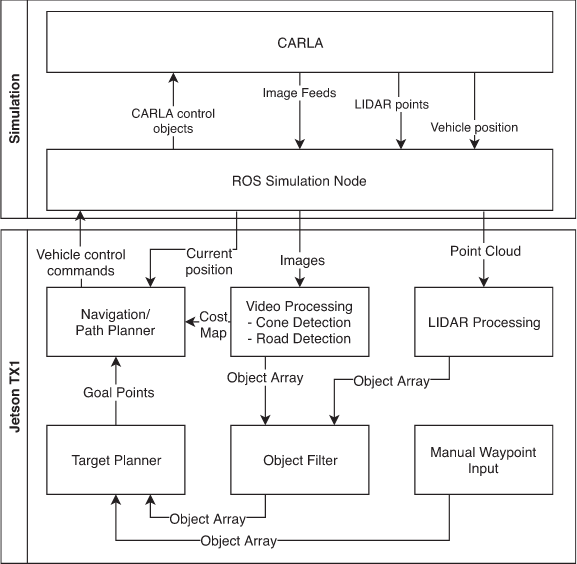
\includegraphics[width=1.0\textwidth]{resources/chapter-2/carla-jetson-arch.png}
    \caption{Arsitektur sistem simulasi \parencite{brogle_CarlaHILS}}
    \label{chapter-2-carla-jetson-arch}
\end{figure}

Hasil eksperimen pada penelitian ini adalah hasil simulasi menggunakan HILS dan
CARLA tidak berbeda jauh dengan keadaan dunia nyata. Selain itu, didapatkan juga
waktu respons pada sistem simulasi lebih cepat dari dunia nyata. Sehingga, dapat
disimpulkan bahwa simulasi HILS dapat dilakukan dan implementasi dengan
menggunakan ROS sudah memberikan hasil yang baik.

Sayangnya, terdapat kendala teknis sehingga pada tugas akhir ini tidak dapat
menggunakan ROS. Kendala teknis itu adalah perbedaan versi sistem operasi yang
menyebabkan versi ROS di komputer AGX/RKB dan komputer SILS tidak saling
kompatibel. Pada komputer AGX/RKB, sistem operasinya adalah Ubuntu 18.04 yang
menggunakan ROS 1 sedangkan komputer SILS menggunakan Ubuntu 20.04 yang
menggunakan ROS 2.
